\documentclass[14pt]{beamer}
\usepackage[T2A]{fontenc}
\usepackage[utf8]{inputenc}
\usepackage[english,russian]{babel}
\usepackage{amssymb,amsfonts,amsmath,mathtext}
\usepackage{cite,enumerate,float,indentfirst}
\usepackage{movie15}

\graphicspath{{images/}}

\usetheme{Berlin}
\usecolortheme{dolphin}

\setbeamercolor{footline}{fg=blue}
\setbeamertemplate{footline}{
  \leavevmode%
  \hbox{%
  \begin{beamercolorbox}[wd=.333333\paperwidth,ht=2.25ex,dp=1ex,center]{}%
	  Лыков Данил, МФТИ
  \end{beamercolorbox}%
  \begin{beamercolorbox}[wd=.333333\paperwidth,ht=2.25ex,dp=1ex,center]{}%
	  Москва, 2018
  \end{beamercolorbox}%
  \begin{beamercolorbox}[wd=.333333\paperwidth,ht=2.25ex,dp=1ex,right]{}%
  стр. \insertframenumber{} из \inserttotalframenumber \hspace*{2ex}
  \end{beamercolorbox}}%
  \vskip0pt%
}

\newcommand{\itemi}{\item[\checkmark]}

\title{\small{Понижение размерности и отбор признаков}}
\author{\small{%
	Данил Лыков
}\\%
\vspace{30pt}%
ФПФЭ МФТИ
\vspace{20pt}%
}
\date{\small{Москва, 2018}}

\begin{document}

\maketitle
\begin{frame}
\frametitle{План}
\begin{itemize}
  \item \textbf{Линейная алгебра} 
	  \begin {itemize}
		\item  Вектора
		\item  Базис
		\item  Преобразование, собственные вектора
	  \end {itemize}
  \item \textbf{Principal Component Ananlysis} 
	  \begin {itemize}
		\item  Постановка задачи
		\item  Реализация
	  \end {itemize}
  \item \textbf{Отбор признаков} 
  \item{Метрики, кросс-валидация} 
\end{itemize}
\end{frame}- 
\begin{frame}
	\frametitle{Вектор}
	Абстрактный объект и операции для которых:
		\pause
	  \begin{itemize}
		  \item \( \alpha (a + b) = \alpha a + \alpha b\)
		  \item \( (\alpha + \beta )a = \alpha a + \beta a\)
			  \vspace{3pt}
			  \pause
		  \item \( a+b = b+a \)
		  \item \( \alpha (\beta a) = (\alpha \beta)a\)
		  \item \( a+(b+c) = (b+a)+c \)
			  \vspace{3pt}
			  \pause
		  \item \( o + a= a \)
		  \item \( a + \overline{a} = o\)
		  \item \( a=1a\)
	  \end{itemize}
\end{frame}

\begin{frame}
\frametitle{Например}
	\vspace{-2em}
	\begin{center}
	   \( \alpha (\beta a) \neq (\alpha \beta)a\)
	\end{center}
    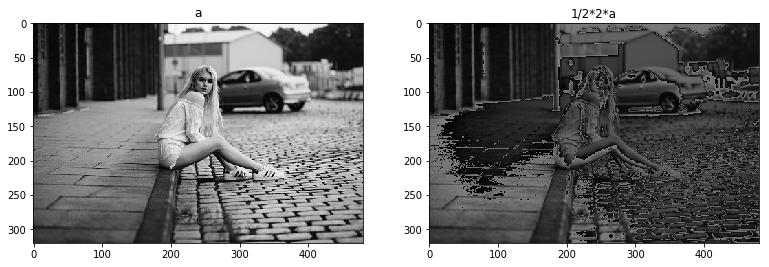
\includegraphics[width=\textwidth]{girl-ok.png}
\end{frame}

% this is commmented>>>
\iffalse
\begin{frame}
	\frametitle{Например #2}
	\vspace{-2em}
	\begin{center}
		  \item \( a+(b+c) \neq (b+a)+c \)\\
    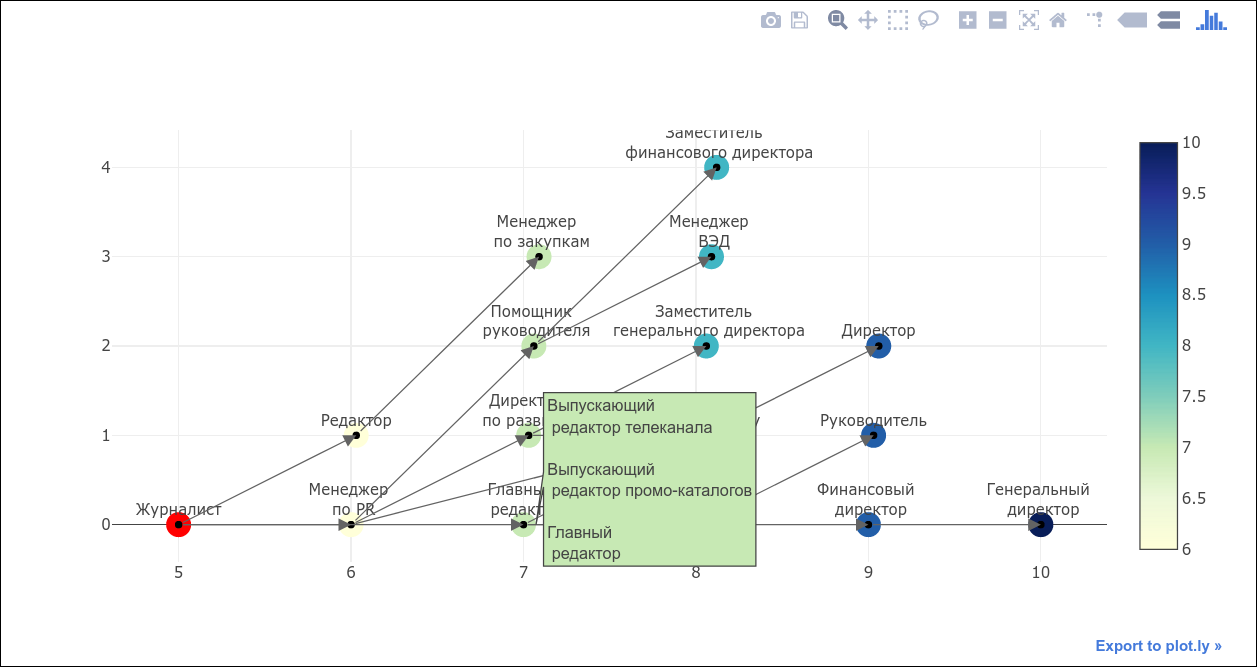
\includegraphics[width=\textwidth]{sum.png}
	\end{center}
\end{frame}
\fi
%<<< this is commmented

\begin{frame}
\frametitle{Базис}
	Множество \( E=\{e_i\}\) для которого:\\
	любой элемент представим в виде суммы элементов из множества $E$ с коэфициентами.\\
	Дают ноль только с нулевыми коэффициентами\\
	\begin{center}
	\( a=\sum_{n=1}^{d} \alpha_n e_n\)\\
	\end{center}
Количество базисных векторов -- размерность пространства
\end{frame}

\begin{frame}
	\vspace{1em}
	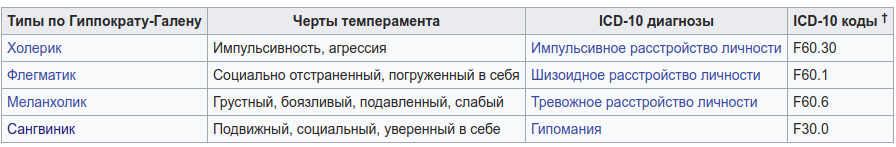
\includegraphics[width=\textwidth]{holer.png}\\
	\vspace{1em}
	
\includegraphics[width=0.2\linewidth]{camb.png}
	\hspace{3em}
	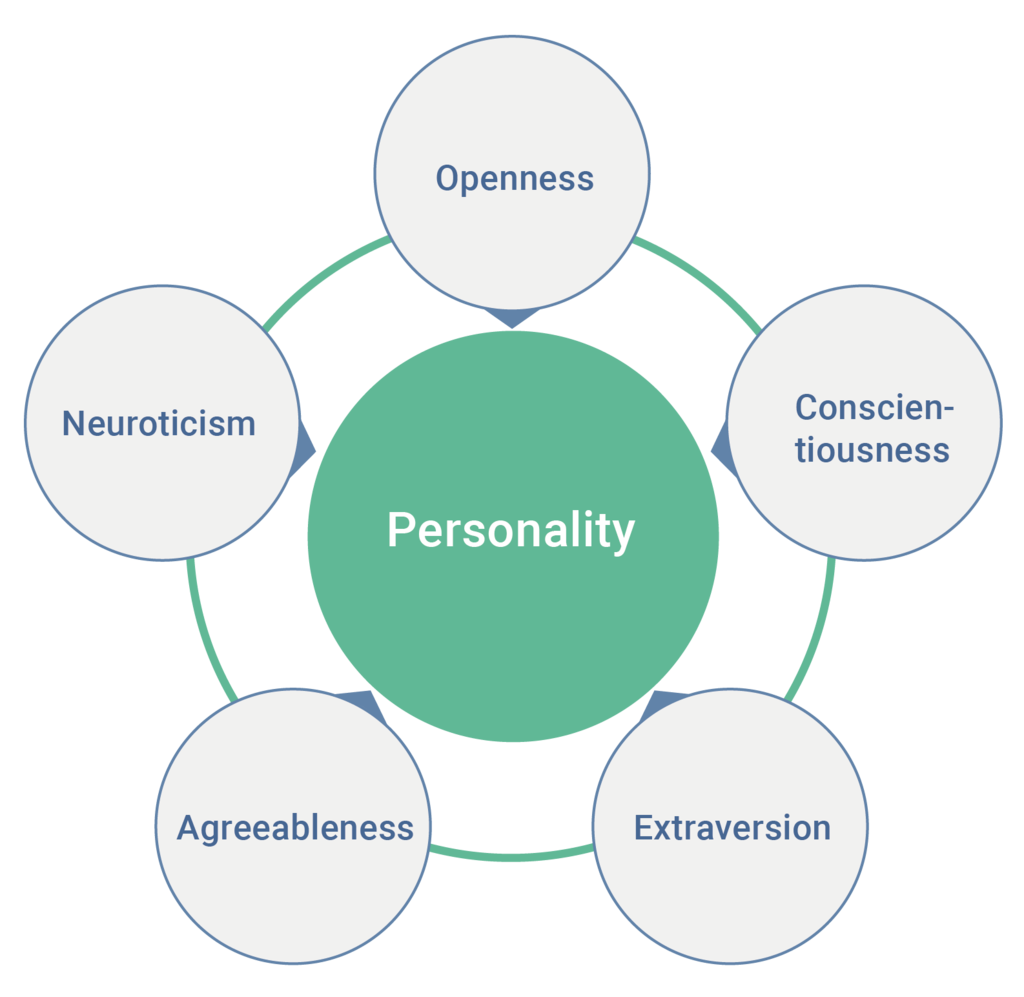
\includegraphics[width=0.2\linewidth]{ocean.png}
	\hspace{3em}
  
\includegraphics[width=0.3\linewidth]{trump.jpeg}\\
	\vspace{1em}
	\textbullet \hspace{1pt} MBTI, OCEAN
\end{frame}

\begin{frame}
\frametitle{Скалярное произведение}
	Любая функция $f: V^2 \mapsto \mathbb{R}$ ($f(a,b)=\alpha$)\\
	для которой:\\
	\pause
	$f(\alpha a+\beta b,c)=\alpha f(a,c) +\beta(b,c)$\\
	$f(a,b)=\overline{f(b,a)}$\\
	$f(a,a)\equiv\langle a,a\rangle \geq0$\\
	\begin{center}
	$	a+b=\sum e\langle e,a \rangle +\sum e\langle e,b \rangle=
	\sum e\langle e,a +b \rangle$
	\end{center}
\end{frame}

\begin{frame}
\frametitle{Principal Component Ananlysis}
	Хотим выбарть другой базис, меньшей размерности, $dim(X)=D, dim(X')=d$\\
	Можно выбрать $\{e_i\}_{i=1}^d$ произвольно,затем оптимизировать \\
	Проекции: $p_i=e_iX$ ($x_j$ -- столбцы, $p_i$ -- строчки)\\
	\begin{center}
  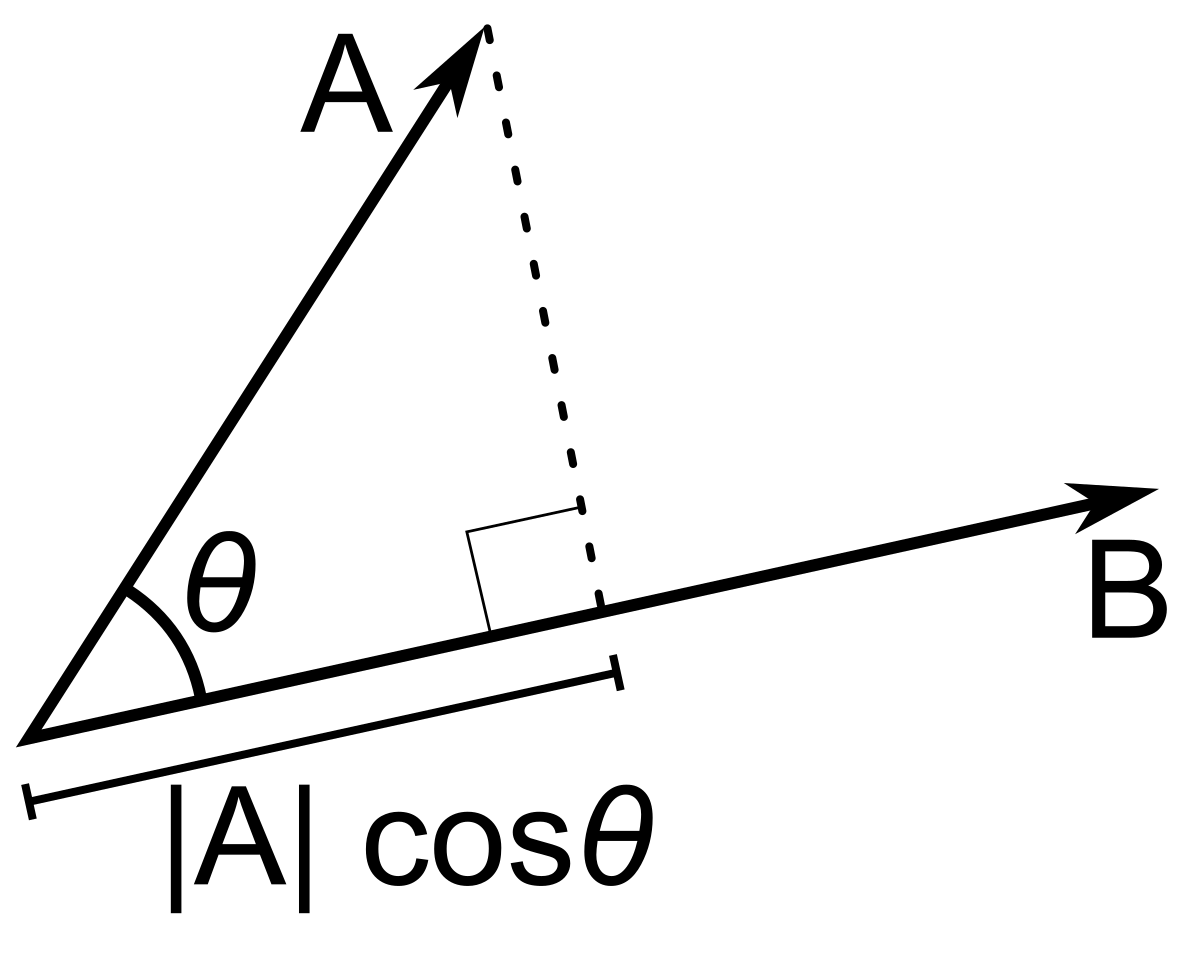
\includegraphics[width=0.4\linewidth]{project.png}\\
	\end{center}
\end{frame}
\begin{frame}
	Цель -- найти такие вектора, проекции $X$ на которые ближе всего исходным данным\\
	Хорошо когда расстояние до вектора меньше -- больше проекция.\\
	\begin{center}
	  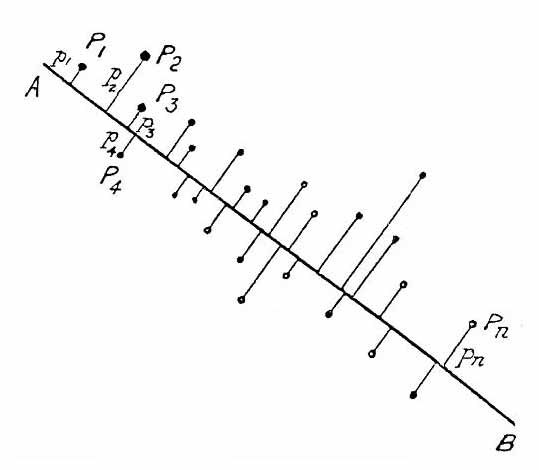
\includegraphics[width=0.45\linewidth]{pearson.jpg}\\
	\end{center}
\end{frame}

\begin{frame}
\frametitle{PCA, Реализация}
	При условии что выборка центрирована, дисперсия: $ p_ip_i^T=\langle e_iX, e_iX \rangle=e_iXX^Te_i^T=\lambda_i$
	Требование: $\langle e_i,e_i \rangle =1 ,E^TE=I$\\
	$e_iXX^Te_i^T=\lambda_i$\\
	Перепишем в немного другом виде\\
	$XX^Te_i^T=\lambda_ie_i^T$\\
	$XX^T$ -- матрица ковариаций\\[1em]
\end{frame}

\begin{frame}
\frametitle{PCA, Реализация}
	$XX^Te_i^T=\lambda_ie_i^T$\\
	Каждой матрице соответствует какое-то преобразование пространства
	(\href{http://setosa.io/ev/eigenvectors-and-eigenvalues/}{\textit{визуализация}})\\

	\begin{center}
	  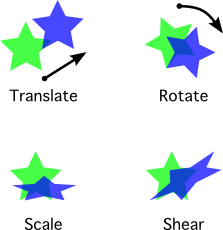
\includegraphics[width=0.3\linewidth]{transform.png}\\
	\end{center}
\end{frame}

\begin{frame}
	Собственные вектора $Wa=\lambda a$\\
	(\href{https://www.desmos.com/calculator/ivo6j1pyex}{\textit{визуализация}})\\
	\begin{center}
	  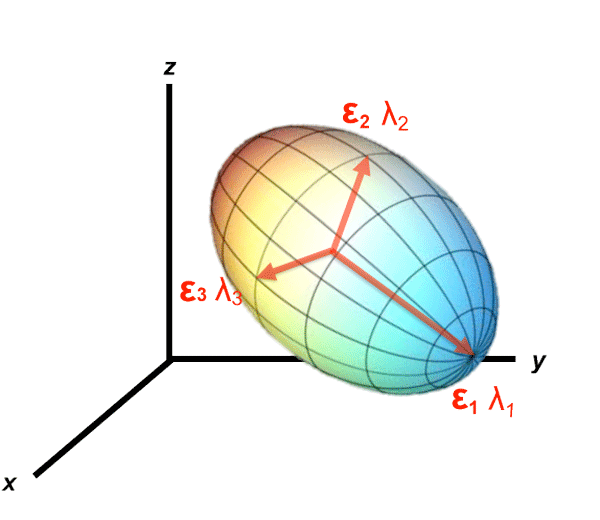
\includegraphics[width=0.5\linewidth]{eigen.png}\\
	\end{center}
\end{frame}

\begin{frame}
\frametitle{PCA, Реализация}
	Как найти?\\
	$X=UDV^T$ Singular Value Decomposition\\
	$U,V$ -- поворот или отражение\\
	$D$ -- все элементы кроме диагональных -- нули\\
	\vspace{1em}
	\pause
	$U$ -- собственные вектора $X^TX$\\
	$V$ -- собственные вектора $XX^T$\\
	$D=diag(\sqrt\lambda_1,\sqrt\lambda_2,..)$ -- диагональная матрица из корней собственных значений\\
\end{frame}

\begin{frame}
\frametitle{PCA, Визуализация}
	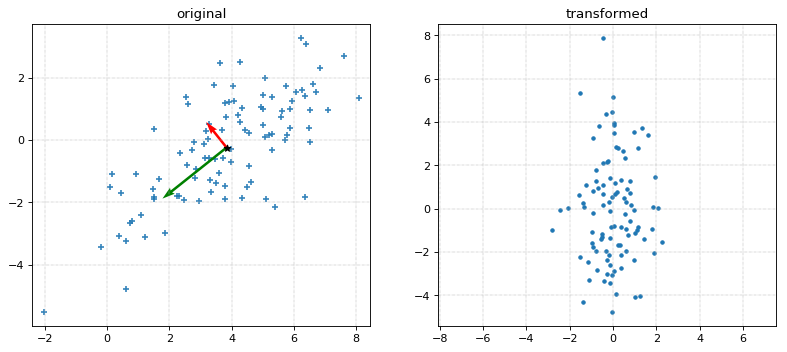
\includegraphics[width=\linewidth]{pca.png}
\end{frame}
\begin{frame}
\frametitle{PCA, Визуализация}
	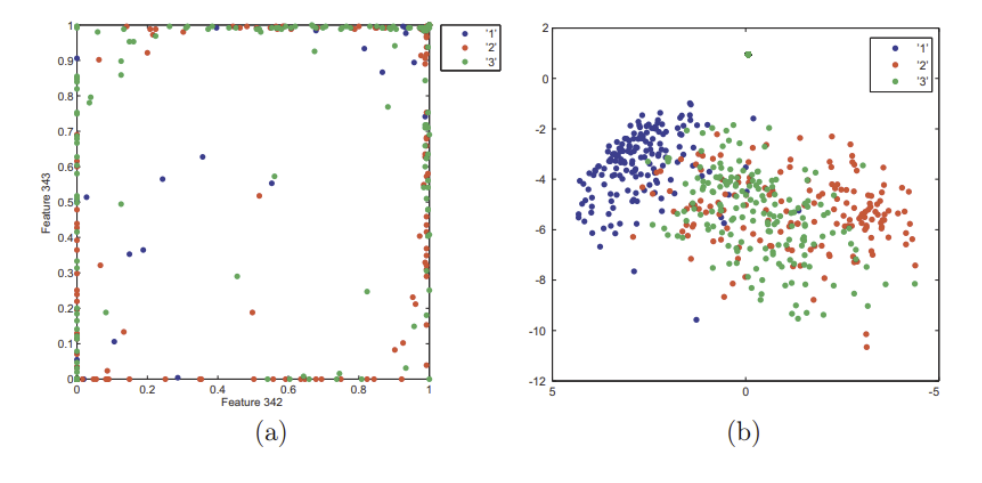
\includegraphics[width=\linewidth]{pca2.png}
\end{frame}

\begin{frame}
\frametitle{Kernel PCA}
	\vspace{-4pt}
	\begin{center}
	$\langle \phi(a),\phi(b) \rangle = K(a,b)$
	\end{center}
	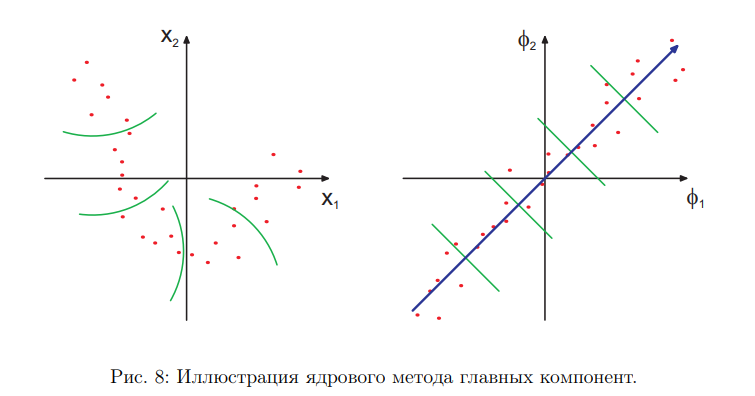
\includegraphics[width=\linewidth]{kerpca.png}
\end{frame}

\begin{frame}
\frametitle{kernel pca}
	\begin{center}
		$k(a,b)=e^{-||a-b||^2}$
	\end{center}
	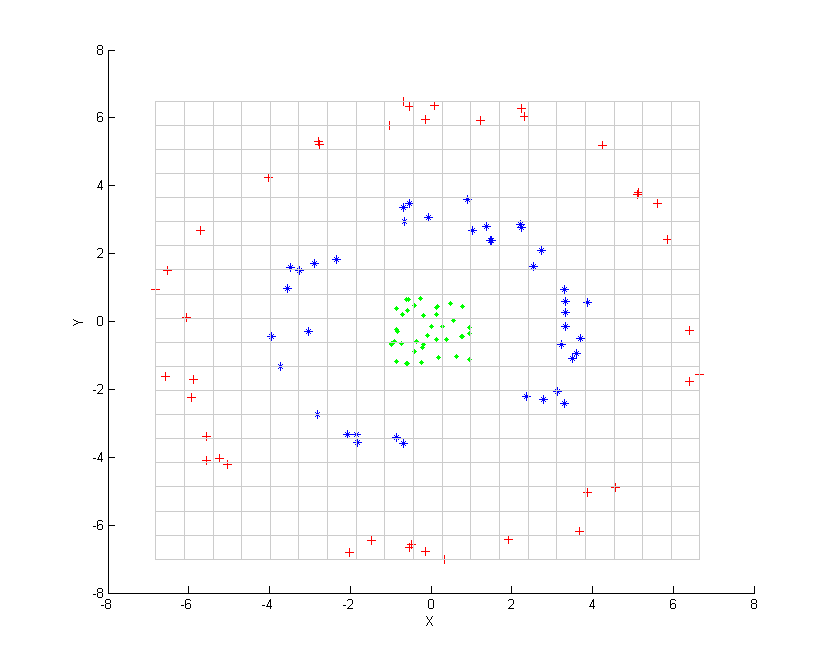
\includegraphics[width=0.5\linewidth]{kerpca1.png}
	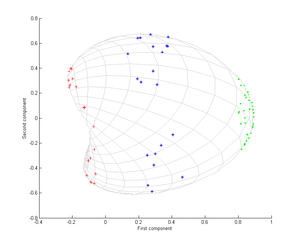
\includegraphics[width=0.5\linewidth]{kerpca2.png}
\end{frame}

\begin{frame}
	\frametitle{Отбор признаков}
	\begin{itemize}
			\item Обучаемся на подмножестве, выбираем лучший скор
			\item Жадный перебор
			\item ADD-DEL
			\item Из данных самой модели
	\end{itemize}
\end{frame}

\begin{frame}
	\frametitle{Кросс-валидация}
	Делим на k частей (фолдов).\\
	Тренируем на k-1 и оцениваем качество модели на одном из них.\\[1em]
	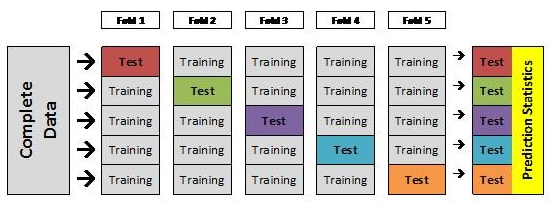
\includegraphics[width=\linewidth]{cv.png}
\end{frame}

\end{document} 
